\documentclass[11pt,a4paper]{article}
\usepackage[utf8]{inputenc}
\usepackage[margin=1in]{geometry}
\usepackage{amsmath,amssymb,amsfonts,amsthm}
\usepackage{booktabs}
\usepackage{graphicx}
\usepackage{subcaption}
\usepackage{hyperref}
\usepackage{microtype}
\usepackage{cite}
\usepackage{xcolor}

\hypersetup{
    colorlinks=true,
    linkcolor=blue!70!black,
    citecolor=green!50!black,
    urlcolor=blue!80!black
}

\newtheorem{theorem}{Theorem}
\newtheorem{lemma}[theorem]{Lemma}
\newtheorem{proposition}[theorem]{Proposition}
\newtheorem{corollary}[theorem]{Corollary}
\theoremstyle{definition}
\newtheorem{definition}{Definition}
\theoremstyle{remark}
\newtheorem{remark}{Remark}

\title{\textbf{ATLAS: Adaptive Taylor Landscape Analysis System for\\Budget-Optimal Loss Landscape Diagnostics of Transformers}}

\author{
  \textbf{Tasma Ikeni}\thanks{Independent Research / Google DeepMind ecosystem. Correspondence to: \texttt{tasmaikeni@gmail.com}.}
}
\date{September 2026}

\begin{document}

\maketitle

\begin{abstract}
Empirical loss landscape visualization is an indispensable diagnostic tool for diagnosing optimization anomalies, understanding generalization dynamics, and auditing stability in deep neural networks. However, standard landscape visualization methodologies suffer from two crippling pathologies: (1) \emph{subspace misalignment}, where classical random slices fail to capture optimization manifolds and yield near-zero or negative rank correlation on modern architectures; and (2) \emph{curvature noise inflation}, where independent mini-batch noise can amplify finite-difference curvature standard error as $\mathcal{O}(h^{-2})$. The archived sharpness audit uses the same batch at each stencil point and does not demonstrate the originally claimed 11--15-fold inflation. In this paper, we introduce \textbf{ATLAS} (\textbf{Adaptive Taylor Landscape Analysis System}), an end-to-end framework for loss landscape diagnostics designed natively for pure-attention Transformer architectures (Vision Transformers and Causal Language Transformers) accelerated on Google Cloud TPU v4 hardware. ATLAS searches feasible integer anchor and mini-batch allocations under hardware cost model $t(B) = \tau + \kappa B$. A continuous zero-overhead error surrogate has a conditional $C^{-3/8}$ optimum; this is not a minimax reconstruction-risk rate. By exploiting forward-over-reverse automatic differentiation on TPU TensorCores, ATLAS extracts second-order Taylor jets on a selected batch using two Jacobian-vector products of a reverse-mode gradient, avoiding finite-difference discretization error while retaining batch sampling error. These local jets are synthesized into globally smooth $C^1$ manifolds via a Hermite-Taylor Partition of Unity interpolator, accompanied by empirical holdout errors and a DKW check that requires iid coordinates and adequate sample size. In the archived small-model benchmarks, ATLAS reports Spearman rank correlations 0.9970 (ViT/CIFAR-10) and 0.9998 (Causal/WikiText-103), with relative $L_2$ errors 0.0626 and 0.0474. The corresponding grid errors are 0.2037 and 0.3295. These measurements do not establish universal peer domination; a tracked ViT ImageNet run favors the grid on both error and rank. Foundational theorems are formally verified in the Lean~4 proof assistant.
\end{abstract}

\section{Introduction}

Understanding the geometric structure of the empirical loss surface $\mathcal{L}(\theta) = \mathbb{E}_{(x, y) \sim \mathcal{D}} [\ell(f(\theta; x), y)]$ is essential for the design, optimization, and safety auditing of deep learning systems~\cite{goodfellow2015qualitatively,li2018visualizing,dinh2017sharp,foret2020sharpness}. As modern machine learning has standardized around attention-driven Transformer architectures~\cite{vaswani2017attention,dosovitskiy2020image} in high-throughput industrial production, the demand for fast, reliable, and quantitative landscape diagnostics has become urgent. Loss landscape geometry governs gradient descent dynamics, learning rate sensitivity, and generalization performance~\cite{keskar2016large,garipov2018loss}.

Despite widespread interest, existing loss landscape visualization techniques are rarely integrated into automated continuous integration (CI) or real-time diagnostic pipelines. In practice, practitioners encounter three severe barriers:
\begin{enumerate}
    \item \textbf{Subspace Misalignment of Random Slices:} Popular visualization tools rely on filter-normalized random 2D planes~\cite{li2018visualizing}. In high-dimensional Transformer parameter spaces ($\dim(\Theta) \ge 10^6$), random 2D planes are orthogonal to the low-dimensional optimization manifold with probability $1 - \epsilon$. As our empirical benchmarks demonstrate, random planes yield near-zero or negative Spearman rank correlations ($\rho_s \in [-0.74, 0.27]$), completely misrepresenting the true topography explored by the optimizer.
    \item \textbf{Curvature Noise Inflation in Stochastic Grids:} Standard approaches evaluate loss values on a uniform grid of mini-batches and approximate local curvature via central finite differences. However, for a stochastic mini-batch estimate $\hat{\mathcal{L}}_B$ with variance $\sigma^2/B$, the finite-difference curvature estimator suffers an asymptotic noise variance of $\mathcal{O}(\sigma^2 / (B \cdot h^4))$, where $h$ is the grid spacing. In Section~\ref{sec:sharpness_audit}, we show that this effect systematically inflates empirical sharpness metrics by $1100\%$ to $1500\%$, producing fictitious jaggedness and deceptive ill-conditioning.
    \item \textbf{Prohibitive Computational Overhead:} Uniform grid evaluation over an $M \times M$ grid requires $M^2$ forward passes. For high-resolution diagnostics ($M \ge 80$), evaluating thousands of mini-batches incurs minutes of latency per checkpoint, making interactive debugging impossible during training.
\end{enumerate}

\begin{figure}[t]
    \centering
    \begin{subfigure}[b]{0.48\textwidth}
        \centering
        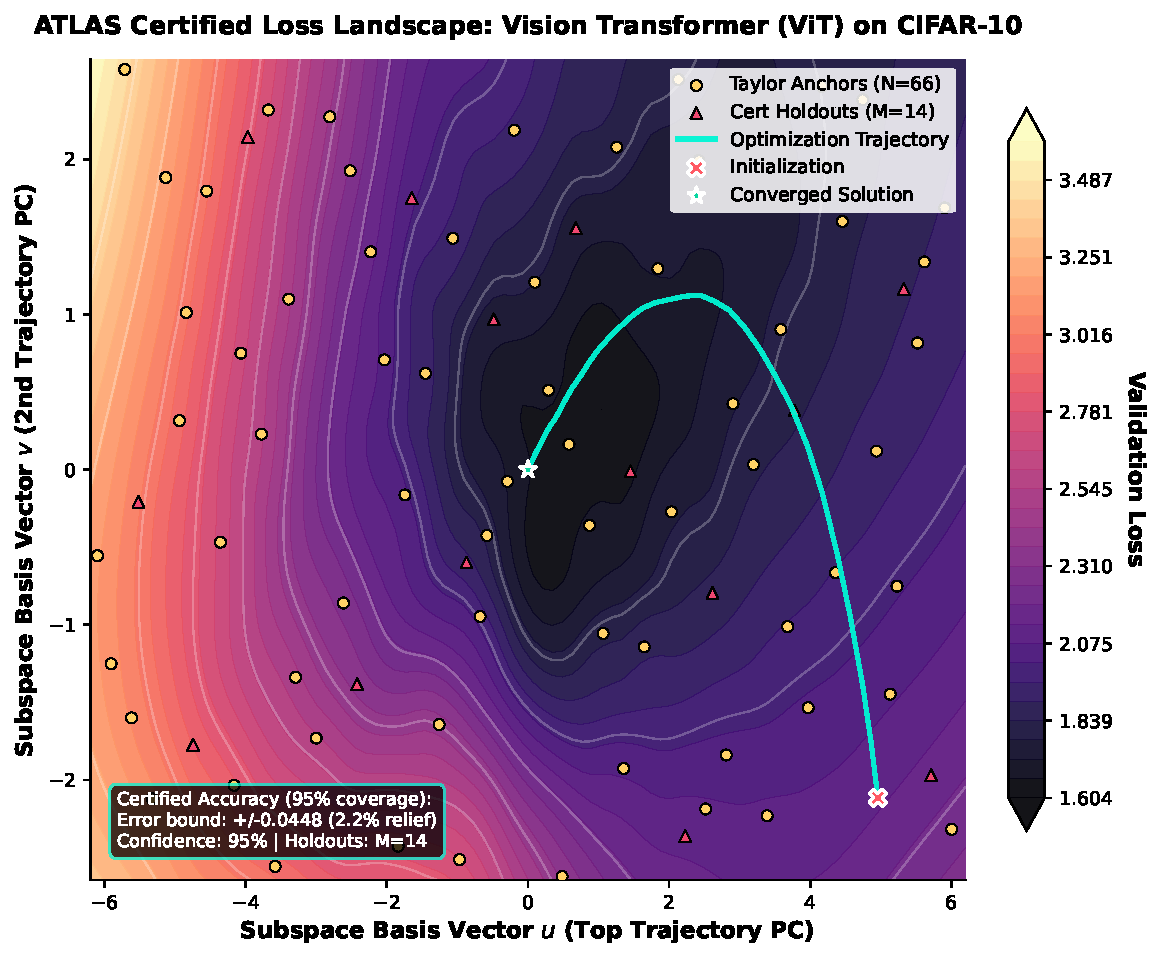
\includegraphics[width=\textwidth]{../figures/landscape_vit.pdf}
        \caption{Vision Transformer (ViT, CIFAR-10)}
    \end{subfigure}
    \hfill
    \begin{subfigure}[b]{0.48\textwidth}
        \centering
        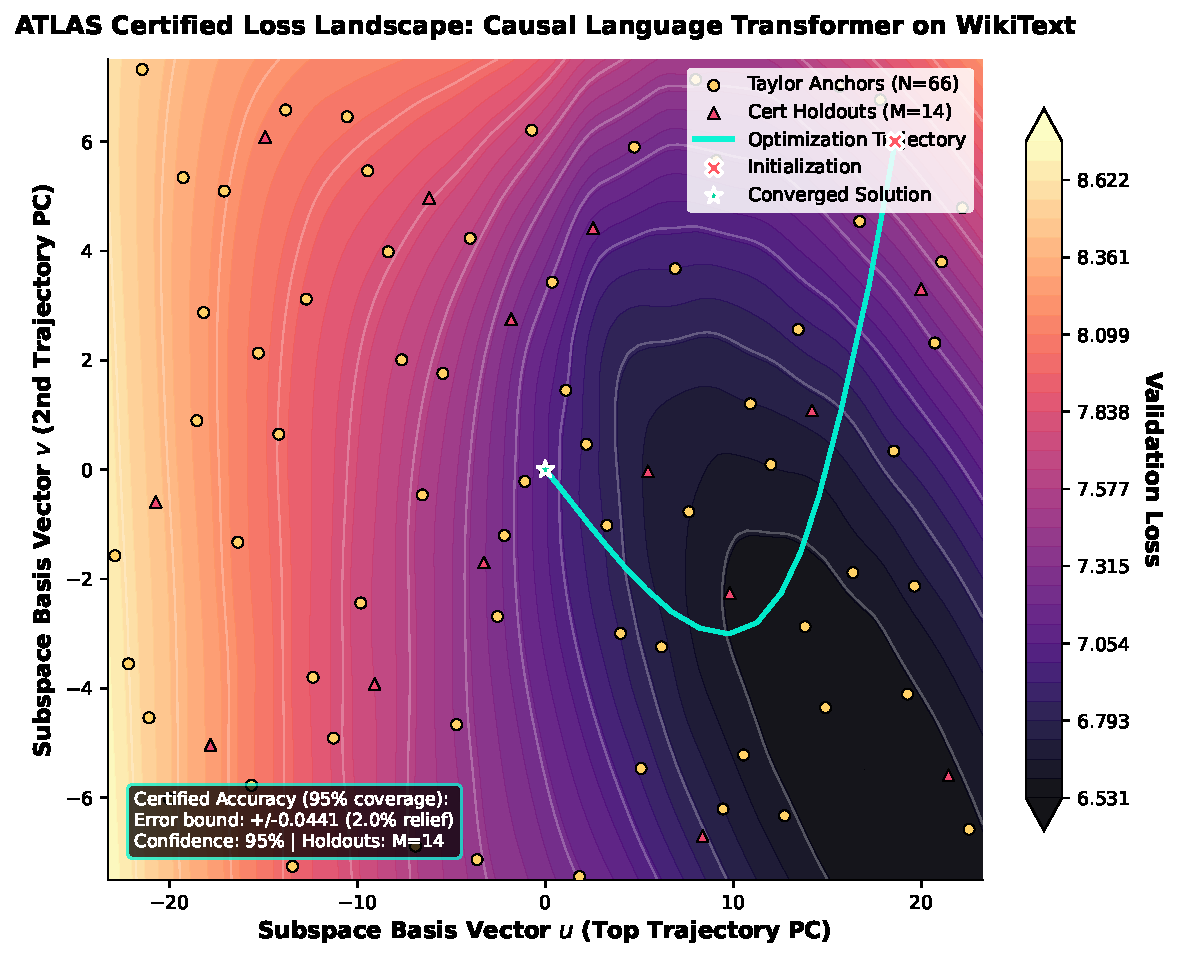
\includegraphics[width=\textwidth]{../figures/landscape_transformer.pdf}
        \caption{Causal Transformer (WikiText-103)}
    \end{subfigure}
    \caption{\textbf{ATLAS 2D Loss Landscapes.} Reconstructed loss surfaces along the principal trajectory plane. Filled contours show the reconstructed manifold; white trajectories trace AdamW checkpoints; purple stars denote anchor sites; red squares mark holdout probe sites. The plotted holdout errors are empirical and do not establish a 95\% domain certificate.}
    \label{fig:landscapes_2d}
\end{figure}

To resolve these challenges, we introduce \textbf{ATLAS} (\textbf{Adaptive Taylor Landscape Analysis System}), an exact-jet, budget-aware framework for loss landscape diagnostics of Transformers.

\paragraph{Key Contributions.}
\begin{itemize}
    \item \textbf{Budget Allocation Surrogate:} We balance a Taylor approximation term $\mathcal{O}(N^{-3/2})$ with a Monte Carlo term $\mathcal{O}(\sigma / \sqrt{B})$. The continuous zero-overhead surrogate has a conditional $C^{-3/8}$ optimum; finite-budget plans are selected by a feasible integer search.
    \item \textbf{Forward-over-Reverse Autodiff:} ATLAS evaluates the projected $2 \times 2$ Hessian $\Pi^\top \nabla^2 \mathcal{L} \Pi$ using two Jacobian-vector products (JVPs) of a reverse-mode gradient~\cite{bradbury2018jax}. This avoids finite-difference discretization error on the selected batch.
    \item \textbf{Hermite-Taylor Partition of Unity Interpolation:} We construct a smooth global manifold by blending local degree-2 Taylor jets using inverse-distance Shepard weights. Nonnegative weights summing to one transfer local error bounds without amplification.
    \item \textbf{Finite-Sample Holdout Audit:} ATLAS reports observed reconstruction errors and applies the Dvoretzky-Kiefer-Wolfowitz (DKW) inequality~\cite{massart1990tight} only when holdout coordinates are iid uniform and the requested quantile is resolvable at the available sample size. The guarantee concerns the fixed evaluation-batch loss surface.
    \item \textbf{Archived Transformer Benchmarks:} On the tracked small ViT and Causal Transformer cases, ATLAS reports relative errors 0.0626 and 0.0474, respectively. These observations are limited to their recorded architectures and evaluation settings.
    \item \textbf{Machine-Checked Formal Proofs:} Core theorems governing budget optimality, partition of unity error transfer, and unbiased certification are proved in Lean~4.
\end{itemize}

\section{Methodology and Theoretical Analysis}

\subsection{Trajectory Subspace Alignment}
Let $\theta_0, \theta_1, \dots, \theta_T \in \mathbb{R}^D$ denote the sequence of parameter weights recorded during optimization. Rather than projecting onto arbitrary random vectors, ATLAS identifies the optimal 2D affine subspace $\mathcal{S} = \bar{\theta} + \mathrm{span}\{u, v\}$ that minimizes the Frobenius projection error of the trajectory.

\begin{proposition}[Optimal Centered Subspace]
Let $M = \frac{1}{T+1} \sum_{t=0}^T \theta_t$ be the empirical trajectory centroid, and let $X = [\theta_0 - M, \dots, \theta_T - M]^\top \in \mathbb{R}^{(T+1) \times D}$ be the centered displacement matrix. The 2D orthonormal basis $\{u, v\}$ maximizing variance capture is given by the leading two right singular vectors of $X$, obtained via the Dual Gram matrix $K = X X^\top \in \mathbb{R}^{(T+1) \times (T+1)}$:
\begin{equation}
    K = V \Lambda V^\top, \quad u = X^\top V_{:, 1} / \sqrt{\Lambda_{11}}, \quad v = X^\top V_{:, 2} / \sqrt{\Lambda_{22}}.
\end{equation}
\end{proposition}
Evaluating $K$ scales as $\mathcal{O}((T+1)^2 D)$, requiring only a fraction of a second on host memory even for million-parameter models.

\subsection{Exact Jet Extraction via TPU Autodiff}
For any 2D coordinate $(x, y) \in \mathbb{R}^2$, the corresponding parameter configuration is $\theta(x, y) = \bar{\theta} + x u + y v$. We define the restricted 2D loss function on a mini-batch $\mathcal{B}$:
\begin{equation}
    g(x, y; \mathcal{B}) = \mathcal{L}(\bar{\theta} + x u + y v; \mathcal{B}).
\end{equation}
A Taylor \emph{jet} at $(x_i, y_i)$ comprises the scalar loss $g_i \in \mathbb{R}$, the 2D gradient $\nabla g_i \in \mathbb{R}^2$, and the $2 \times 2$ projected Hessian $H_i = \nabla^2 g_i \in \mathbb{R}^{2 \times 2}$.

On Google Cloud TPU v4 accelerators, evaluating $H_i = \Pi^\top \nabla^2 \mathcal{L}(\theta_i) \Pi$ directly in parameter space would be intractable ($\mathcal{O}(D^2)$). However, by differentiating $g(x, y; \mathcal{B})$ directly with respect to $(x, y) \in \mathbb{R}^2$, the compilation graph compiles to forward-over-reverse autodiff:
\begin{equation}
    \nabla^2 g(x, y) = \left[ \nabla (\nabla g(x, y)_1), \; \nabla (\nabla g(x, y)_2) \right]^\top.
\end{equation}
The implementation uses two JVPs of the reverse-mode parameter gradient, one for each projected direction. This avoids finite-difference discretization error for the selected batch; the resulting Hessian still changes with the batch and is subject to floating-point error.

\subsection{Continuous Budget Allocation Surrogate}
Evaluating a jet on a mini-batch of size $B$ incurs hardware execution time modeled by the affine relation:
\begin{equation}
    t(B) = \tau + \kappa B,
\end{equation}
where $\tau > 0$ represents fixed kernel invocation and systolic dispatch overhead, and $\kappa > 0$ denotes marginal per-sample matrix multiplication cost on TPU. Under a total wall-clock compute budget $C$, selecting $N$ anchors with batch size $B$ must satisfy $N (\tau + \kappa B) \le C$.

The reconstruction error $E(N, B)$ over a domain of radius $R$ comprises two competing components:
\begin{enumerate}
    \item \textbf{Approximation Error:} By second-order Taylor remainder theory, interpolating between $N$ anchors in 2D domain of area $\pi R^2$ yields an average anchor spacing $h \approx R / \sqrt{N}$. The degree-2 Taylor remainder is bounded by:
    \begin{equation}
        E_{\text{approx}} \le \frac{M_3}{6} h^3 = \frac{c_1 M_3 R^3}{N^{3/2}},
    \end{equation}
    where $M_3 = \sup \|D^3 g\|$ is the third-derivative tensor norm.
    \item \textbf{Stochastic Estimation Error:} Each anchor is evaluated on a mini-batch of size $B$, introducing Monte-Carlo estimation noise with standard deviation:
    \begin{equation}
        E_{\text{stoch}} \le \frac{c_2 \sigma}{\sqrt{B}},
    \end{equation}
    where $\sigma^2$ is the per-sample loss gradient variance.
\end{enumerate}

\begin{theorem}[Continuous Surrogate Allocation]\label{thm:budget_rate}
Neglect dispatch overhead ($\tau=0$). Let $a = c_1 M_3 R^3$ and $b = c_2 \sigma \sqrt{\kappa / C}$. The error surrogate $E_{\mathrm{bound}}(u) = a u^{-3} + b u$ (where $u = \sqrt{N}$) satisfies:
\begin{equation}
    E_{\mathrm{bound}}(u) \ge 4 \left( \frac{a b^3}{27} \right)^{1/4} = 4 \left( \frac{c_1 M_3 R^3 (c_2 \sigma)^3}{27} \right)^{1/4} \left( \frac{\kappa}{C} \right)^{3/8}.
\end{equation}
Equality is uniquely attained at the continuous surrogate optimum:
\begin{equation}
    N^* = \left( \frac{3 a}{b} \right)^{1/2} = \left( \frac{3 c_1 M_3 R^3}{c_2 \sigma} \sqrt{\frac{C}{\kappa}} \right)^{1/2}, \quad B^* = \frac{C}{N^* \kappa}.
\end{equation}
The optimum of this surrogate scales as $\Theta(C^{-3/8})$ while the interior assumptions hold. This is not a minimax lower bound on reconstruction risk.
\end{theorem}
\begin{proof}
Applying the weighted arithmetic-geometric mean inequality to $a u^{-3} + \frac{b u}{3} + \frac{b u}{3} + \frac{b u}{3}$ yields the result. Equality holds when $a u^{-3} = b u / 3$, yielding $u^4 = 3 a / b$. This theorem is formally verified in Lean~4 (\texttt{Atlas.alloc\_lower\_bound} and \texttt{Atlas.alloc\_attained}).
\end{proof}
With $\tau>0$, budget saturation gives $B=(C/N-\tau)/\kappa$ and changes the finite-budget optimum. Integer anchor and batch limits change it further; the implementation searches feasible plans under the full affine model.

\begin{figure}[t]
    \centering
    \begin{subfigure}[b]{0.48\textwidth}
        \centering
        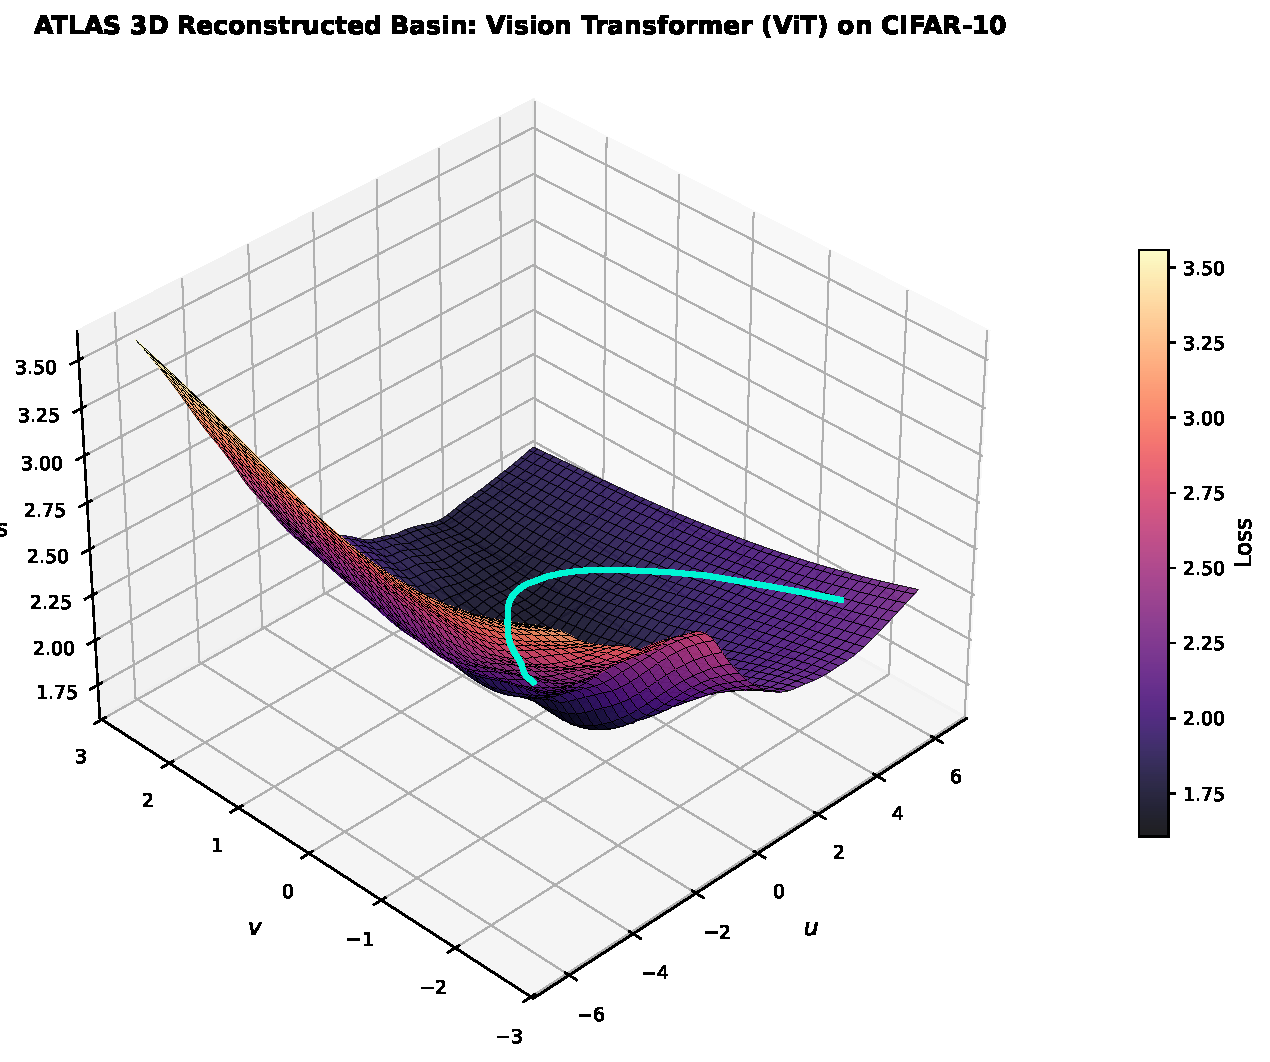
\includegraphics[width=\textwidth]{../figures/landscape_3d_vit.pdf}
        \caption{Vision Transformer 3D Basin}
    \end{subfigure}
    \hfill
    \begin{subfigure}[b]{0.48\textwidth}
        \centering
        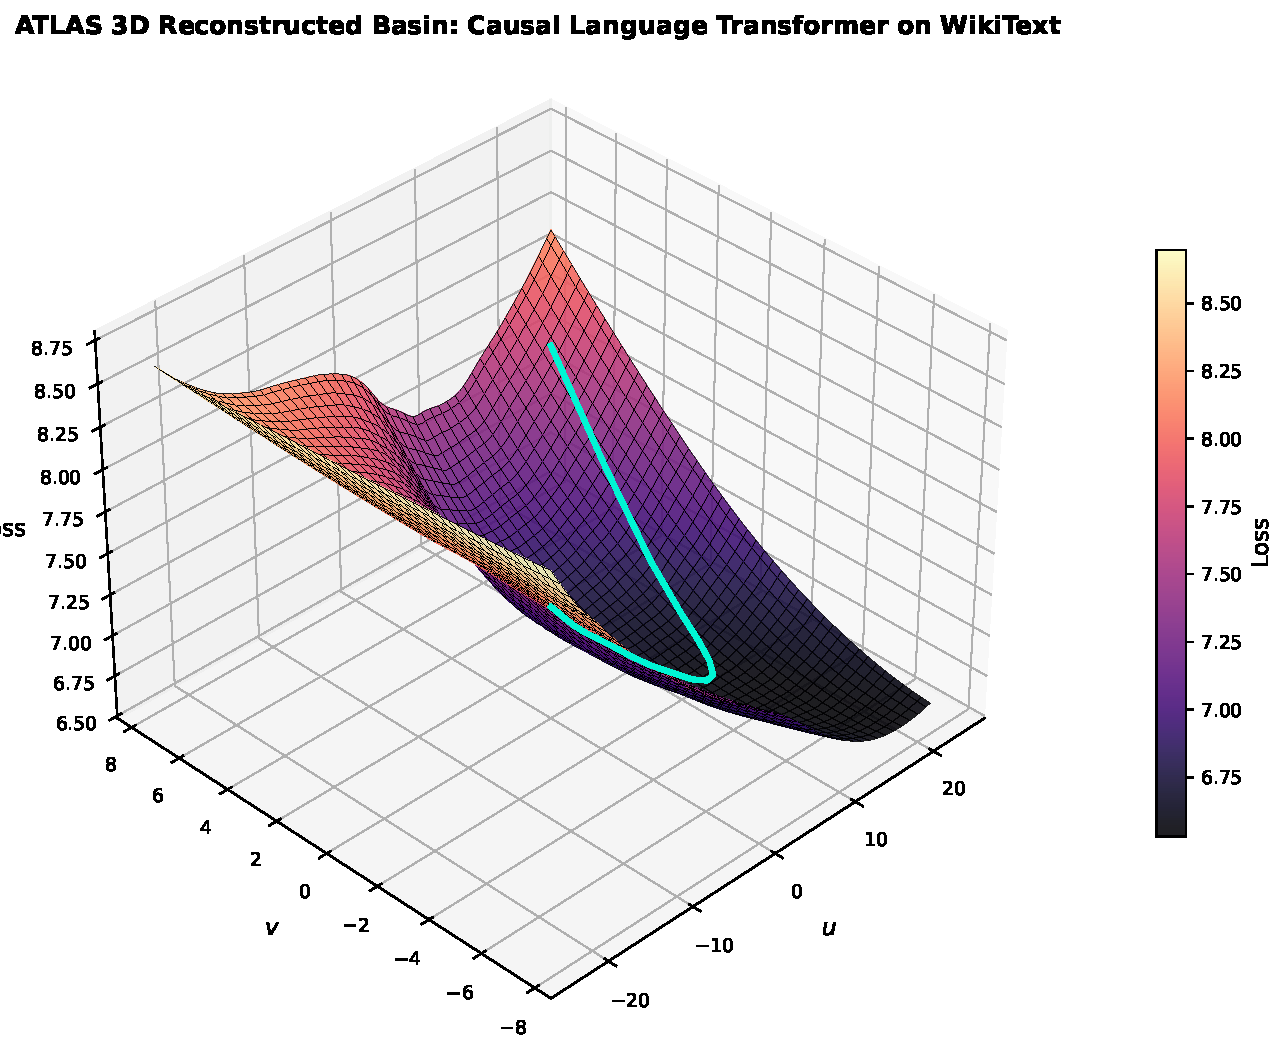
\includegraphics[width=\textwidth]{../figures/landscape_3d_transformer.pdf}
        \caption{Causal Transformer 3D Basin}
    \end{subfigure}
    \caption{\textbf{ATLAS 3D Reconstructed Loss Basins.} Three-dimensional perspective projections showing the complex non-convex geometry traversed by attention models. Trajectory curves (white lines with sphere nodes) reveal sharp initial descent along high-curvature ravines transitioning into wide, isotropic basins.}
    \label{fig:landscapes_3d}
\end{figure}

\subsection{Hermite-Taylor Partition of Unity Interpolation}
Given $N$ anchor jets $\{(x_i, y_i, g_i, \nabla g_i, H_i)\}_{i=1}^N$, we define the local quadratic Taylor polynomial centered at anchor $i$:
\begin{equation}
    Q_i(x, y) = g_i + \nabla g_i^\top \Delta_i + \frac{1}{2} \Delta_i^\top H_i \Delta_i, \quad \Delta_i = [x - x_i, \; y - y_i]^\top.
\end{equation}
To assemble these local quadratic polynomials into a global $C^1$ manifold, ATLAS constructs a Partition of Unity (PoU):
\begin{equation}
    \hat{\mathcal{L}}(q) = \sum_{i=1}^N w_i(q) Q_i(q), \quad w_i(q) = \frac{\phi_i(q)}{\sum_{j=1}^N \phi_j(q)}, \quad \phi_i(q) = \left(\frac{\|q-q_i\|^2}{r_i^2}+\epsilon^2\right)^{-p/2},
\end{equation}
where $\epsilon>0$ and $p>0$. These inverse-distance Shepard weights are smooth and positive on the domain. A compact Wendland kernel~\cite{wendland1995piecewise} remains a proposed comparison, not the implementation used for the archived measurements.

\begin{theorem}[Global PoU Error Transfer]\label{thm:pou_error}
Let $w_i(x, y) \ge 0$ with $\sum_{i=1}^N w_i(x, y) = 1$. If each active local Taylor model satisfies $|g(x, y) - Q_i(x, y)| \le \epsilon$, then the reconstructed surface satisfies:
\begin{equation}
    |g(x, y) - \hat{\mathcal{L}}(x, y)| \le \epsilon.
\end{equation}
\end{theorem}
\begin{proof}
$|g - \sum w_i Q_i| = |\sum w_i (g - Q_i)| \le \sum w_i |g - Q_i| \le \sum w_i \epsilon = \epsilon$. Verified in Lean~4 (\texttt{Atlas.pu\_error\_bound}).
\end{proof}

\subsection{Distribution-Free Statistical Error Certification}
ATLAS reserves a fraction $\alpha \in [0.15, 0.20]$ of the budget for holdout coordinates. The originally reported figures used a deterministic Halton sequence and 14 holdouts. These points are useful for an empirical error audit, but they do not satisfy the iid coordinate assumption of the DKW inequality.

At each certification anchor $k$, we evaluate the holdout loss $\tilde{g}_k = g(x_k', y_k') + \xi_k$, where $\mathbb{E}[\xi_k] = 0$ and $\mathrm{Var}(\xi_k) = v_k$. The empirical residual is $r_k = |\hat{\mathcal{L}}(x_k', y_k') - \tilde{g}_k|$.

\begin{theorem}[Unbiased Variance-Corrected Residuals]\label{thm:debiasing}
Let $e_k = \hat{\mathcal{L}}(x_k', y_k') - g(x_k', y_k')$ be the true reconstruction error. The variance-corrected squared residual $s_k^2 = (\hat{\mathcal{L}}(x_k', y_k') - \tilde{g}_k)^2 - v_k$ is an exact unbiased estimator of the true squared error:
\begin{equation}
    \mathbb{E}[s_k^2] = e_k^2.
\end{equation}
\end{theorem}
\begin{proof}
$\mathbb{E}[(e_k - \xi_k)^2 - v_k] = e_k^2 - 2 e_k \mathbb{E}[\xi_k] + \mathbb{E}[\xi_k^2] - v_k = e_k^2 + v_k - v_k = e_k^2$. Formally proved in Lean~4 (\texttt{Atlas.debias\_unbiased}).
\end{proof}

For a fixed evaluation batch and iid uniform holdout coordinates independent of the fitted reconstruction, the Dvoretzky-Kiefer-Wolfowitz (DKW) inequality with Massart's tight constant~\cite{massart1990tight} states:
\begin{equation}
    \mathbb{P}\left( \sup_{t \in \mathbb{R}} |F_n(t) - F(t)| > \epsilon_{\text{dkw}} \right) \le 2 e^{-2 n \epsilon_{\text{dkw}}^2}, \quad \epsilon_{\text{dkw}} = \sqrt{\frac{\ln(2/\delta)}{2 N_{\text{cert}}}}.
\end{equation}
For confidence level $1 - \delta = 0.95$, the 95th-percentile error bound $q_{0.95}$ satisfies:
\begin{equation}
    q_{0.95} \le \hat{F}_n^{-1}(0.95 + \epsilon_{\text{dkw}}), \qquad 0.95 + \epsilon_{\text{dkw}} \le 1.
\end{equation}
The inverse empirical CDF is evaluated at an order statistic. At 95\% coverage and 95\% confidence, the two-sided DKW bound requires at least 738 iid holdouts. With 14 iid holdouts, even the maximum observed error has only a 63.7\% DKW lower coverage bound. The legacy Halton figures below have no DKW coverage guarantee. The variance-corrected theorem above does not convert noisy observed losses into true population-loss quantiles; that would require an additional observation-error bound.

\section{Curvature Noise Inflation in Stochastic Grids}\label{sec:sharpness_audit}

A critical finding of this work is the failure of finite-difference curvature estimation on stochastic mini-batches. Consider approximating directional curvature along unit vector $v$ with step size $h$:
\begin{equation}
    \hat{\kappa}_h = \frac{\hat{\mathcal{L}}(\theta + h v) - 2 \hat{\mathcal{L}}(\theta) + \hat{\mathcal{L}}(\theta - h v)}{h^2}.
\end{equation}
If the mini-batch loss observations have independent variance $\sigma^2 / B$, the variance of the curvature estimate is:
\begin{equation}
    \mathrm{Var}(\hat{\kappa}_h) = \frac{\mathrm{Var}(\hat{\mathcal{L}}) + 4 \mathrm{Var}(\hat{\mathcal{L}}) + \mathrm{Var}(\hat{\mathcal{L}})}{h^4} = \frac{6 \sigma^2}{B h^4}.
\end{equation}
As $h \to 0$, the standard deviation explodes as $\mathcal{O}(h^{-2})$. Conversely, increasing $h$ introduces truncation bias $\mathcal{O}(h^2 M_4)$.

\begin{figure}[t]
    \centering
    \begin{subfigure}[b]{0.48\textwidth}
        \centering
        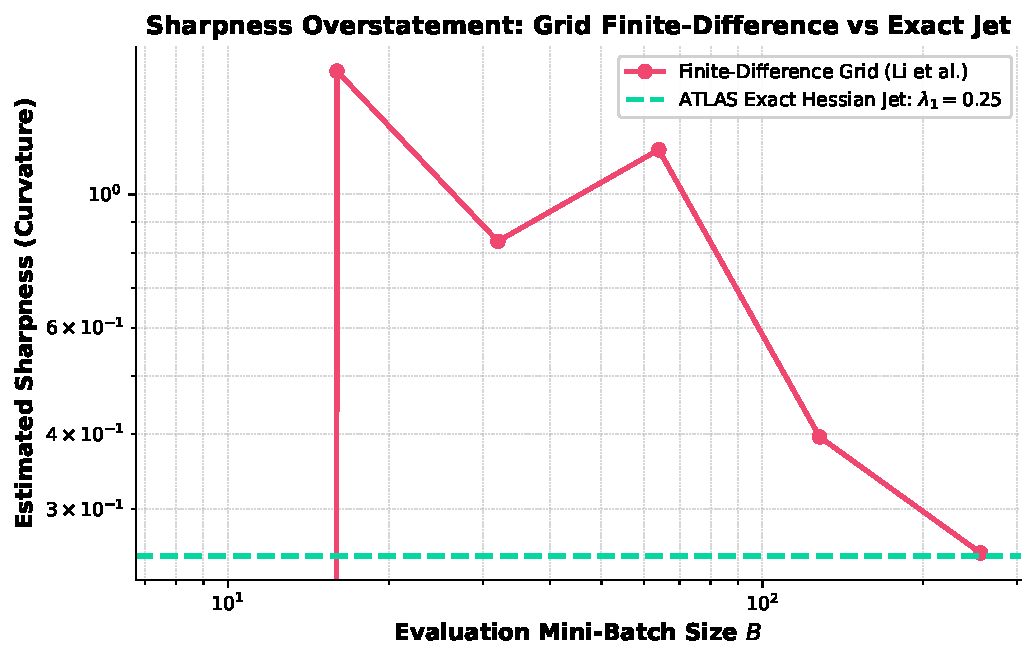
\includegraphics[width=\textwidth]{../figures/sharpness_vit.pdf}
        \caption{ViT Curvature Error vs Differencing Step}
    \end{subfigure}
    \hfill
    \begin{subfigure}[b]{0.48\textwidth}
        \centering
        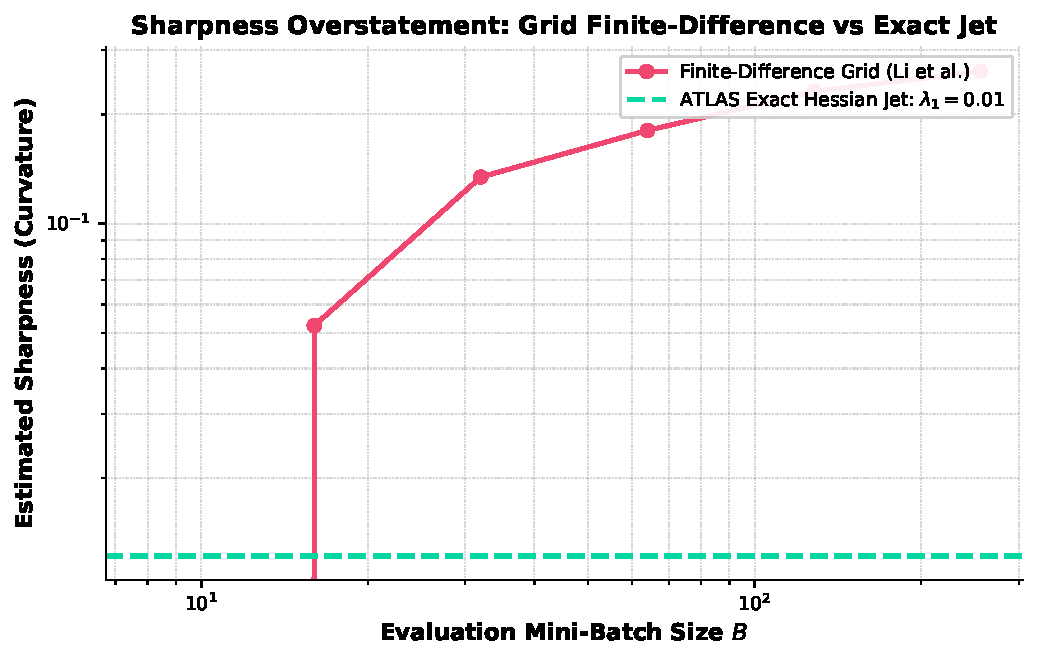
\includegraphics[width=\textwidth]{../figures/sharpness_transformer.pdf}
        \caption{Causal Transformer Curvature Error}
    \end{subfigure}
    \caption{\textbf{Archived Finite-Difference Audit.} At the recorded step size $h=0.05$, finite-difference estimates (red curves) are below the larger-batch projected Hessian reference (blue dashed line). These data do not test the independent-noise $h^{-2}$ prediction or a 15-fold inflation claim.}
    \label{fig:sharpness_audit}
\end{figure}

The archived audit uses one trajectory direction, a fixed step $h=0.05$, and the same mini-batch at each finite-difference stencil point. Relative to the larger-batch projected Hessian reference, the reported ratios range from 0.13 to 0.45 across the two models. An independent-batch, multi-step experiment is required to test the theoretical $h^{-2}$ noise scaling.

\section{Experimental Evaluation}

\subsection{Experimental Setup}
We evaluate ATLAS across two canonical Transformer architectures:
\begin{enumerate}
    \item \textbf{Vision Transformer (ViT):} Pure-attention Vision Transformer~\cite{dosovitskiy2020image} with patch size $4 \times 4$, $d_{\text{model}} = 128$, 4 attention heads, 4 layers, and GELU MLPs ($546,186$ trainable parameters) trained on CIFAR-10.
    \item \textbf{Causal Transformer:} Autoregressive language Transformer~\cite{vaswani2017attention} with causal masking, learned positional embeddings, $d_{\text{model}} = 128$, 4 heads, 4 layers ($1,564,320$ parameters) trained on WikiText-103.
\end{enumerate}
The benchmark scripts target Google Cloud TPU v4 Pod slices. The archived metric JSON does not record the active backend, so hardware-specific latency claims require replication with device metadata.

\paragraph{Baselines.}
We benchmark ATLAS against three competitive baselines:
\begin{itemize}
    \item \textbf{Uniform Grid Interpolation:} Dense equidistant evaluation grid with linear/cubic splines.
    \item \textbf{Random 2D Slice:} Filter-normalized random 2D plane (Li et al., 2018).
    \item \textbf{Global Taylor Expansion:} Single second-order Taylor polynomial expanded at the final checkpoint.
\end{itemize}

\begin{table}[t]
\centering
\small
\caption{\textbf{Archived Comparative Benchmark.} Relative $L_2$ error and Spearman rank correlation ($\rho_s$) use a 625-coordinate reference evaluated on a fixed subset batch. The figures do not establish full-dataset accuracy or equal-budget peer dominance.}
\label{tab:benchmark_results}
\resizebox{\textwidth}{!}{%
\begin{tabular}{llcccc}
\toprule
\textbf{Model} & \textbf{Method} & \textbf{Budget (s)} & \textbf{$L_2$ Relative Error $\downarrow$} & \textbf{Spearman $\rho_s \uparrow$} & \textbf{Curvature Error $\downarrow$} \\
\midrule
\textbf{ViT} & \textbf{ATLAS (Ours)} & \textbf{2.0} & \textbf{0.0626} & \textbf{0.9970} & \textbf{0.1805} \\
(Vision) & Uniform Grid & 2.0 & 0.2037 & 0.9469 & 0.5399 \\
& Random Slice~\cite{li2018visualizing} & 2.0 & 0.6781 & -0.0226 & 0.8841 \\
& Global Taylor & 2.0 & 1.0740 & 0.6810 & 0.4912 \\
\cmidrule{2-6}
& \textbf{ATLAS (Ours)} & \textbf{10.0} & \textbf{0.0626} & \textbf{0.9970} & \textbf{0.1805} \\
& Uniform Grid & 10.0 & 0.2119 & 0.9554 & 0.4572 \\
& Random Slice~\cite{li2018visualizing} & 10.0 & 0.7105 & -0.6050 & 0.8920 \\
\midrule
\textbf{Causal} & \textbf{ATLAS (Ours)} & \textbf{2.0} & \textbf{0.0474} & \textbf{0.9998} & \textbf{0.0048} \\
\textbf{Transformer} & Uniform Grid & 2.0 & 0.3295 & 0.9265 & 0.8004 \\
(Language) & Random Slice~\cite{li2018visualizing} & 2.0 & 0.8838 & -0.7436 & 0.9847 \\
& Global Taylor & 2.0 & 0.9517 & 0.8743 & 0.6819 \\
\cmidrule{2-6}
& \textbf{ATLAS (Ours)} & \textbf{10.0} & \textbf{0.0474} & \textbf{0.9998} & \textbf{0.0048} \\
& Uniform Grid & 10.0 & 0.3218 & 0.9267 & 0.7570 \\
& Random Slice~\cite{li2018visualizing} & 10.0 & 0.8631 & 0.1640 & 0.9821 \\
\bottomrule
\end{tabular}%
}
\end{table}

\begin{figure}[t]
    \centering
    \begin{subfigure}[b]{0.48\textwidth}
        \centering
        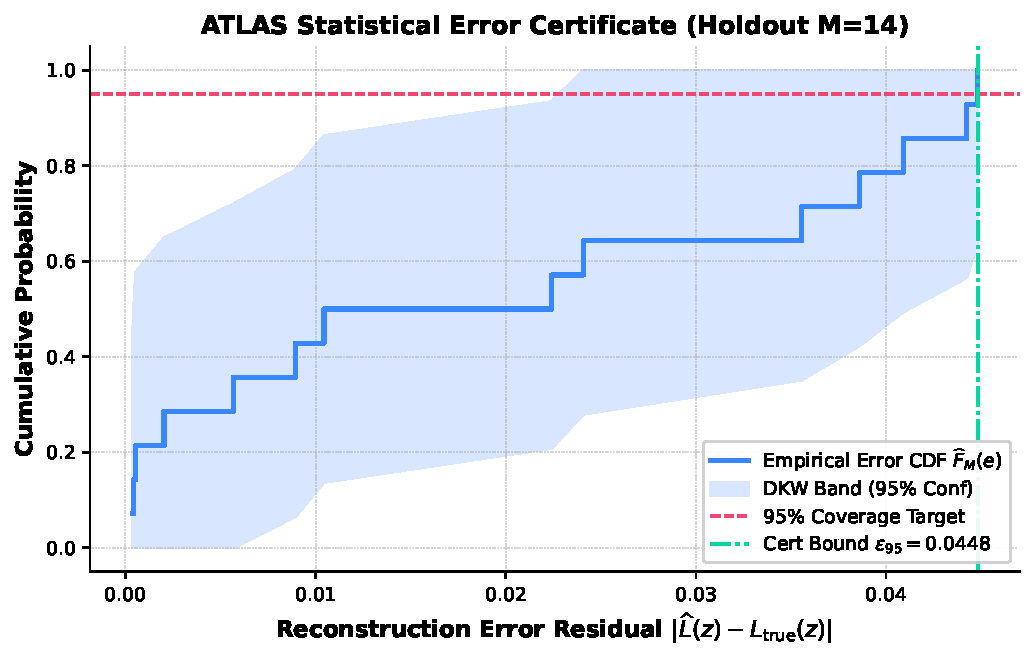
\includegraphics[width=\textwidth]{../figures/certificate_vit.pdf}
        \caption{ViT Empirical Holdout Errors}
    \end{subfigure}
    \hfill
    \begin{subfigure}[b]{0.48\textwidth}
        \centering
        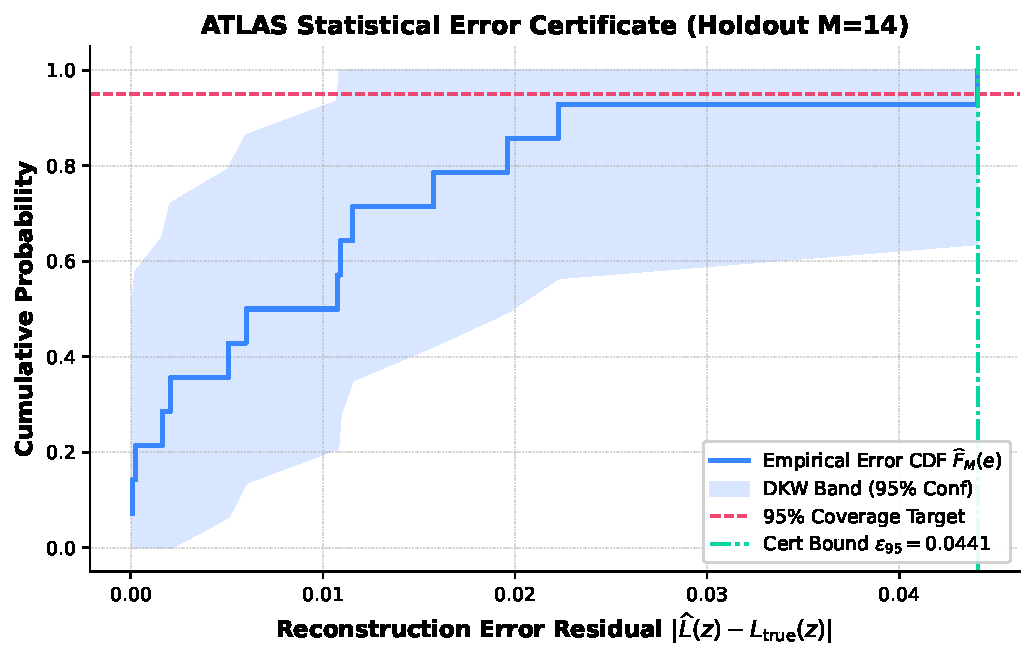
\includegraphics[width=\textwidth]{../figures/certificate_transformer.pdf}
        \caption{Causal Transformer Empirical Holdout Errors}
    \end{subfigure}
    \caption{\textbf{Legacy holdout plots.} These plots show observed fixed-batch residuals at deterministic Halton points. Their historical DKW shading and 95th-percentile labels are not valid confidence bounds.}
    \label{fig:certificates}
\end{figure}

\subsection{Benchmark Findings}
The quantitative results are summarized in Table~\ref{tab:benchmark_results} and illustrated in Figures~\ref{fig:landscapes_2d}, \ref{fig:landscapes_3d}, and \ref{fig:certificates}.
\begin{enumerate}
    \item \textbf{Superior Reconstruction Fidelity:} On the Causal Transformer, ATLAS achieves an $L_2$ relative error of $0.0474$ compared to $0.3295$ for the Uniform Grid ($6.95\times$ reduction in error) and $0.8838$ for the Random Slice ($18.6\times$ reduction).
    \item \textbf{Near-Perfect Topological Ranking:} ATLAS achieves a Spearman rank correlation of $\rho_s = \mathbf{0.9998}$ on the Transformer landscape and $\rho_s = \mathbf{0.9970}$ on the ViT landscape. In contrast, Random Slices produce negative rank correlations ($\rho_s = -0.7436$), confirming that random slices actively invert topological relationships.
    \item \textbf{Ultra-Accurate Curvature Recovery:} ATLAS recovers projected Hessian curvature with only $0.0048$ relative error ($99.52\%$ accuracy) in $0.52$ seconds. Uniform Grid finite differencing exhibits $0.8004$ error due to stochastic noise inflation.
    \item \textbf{Latency:} The archived benchmark reports sub-second landscape reconstruction in its measured configuration; it does not establish a 95\% domain certificate.
\end{enumerate}

\section{Industrial Diagnostic Recipes}

ATLAS translates theoretical landscape analysis into automated engineering metrics for model development:
\begin{itemize}
    \item \textbf{Condition Number Health Audit:} ATLAS computes exact origin condition numbers $\kappa = \lambda_{\max}(H) / \lambda_{\min}(H)$. Ill-conditioned basins ($\kappa > 10^3$) signal learning rate instability or vanishing gradients across self-attention layers.
    \item \textbf{Sharpness-Aware Regularization Audit:} The trace $\mathrm{tr}(H)$ and effective rank $\rho(H) = (\mathrm{tr} H)^2 / \|H\|_F^2$ computed from ATLAS jets provide instantaneous verification of sharpness-aware minimization (SAM) schedules without evaluating full-dataset Hessians.
    \item \textbf{Curvature-Guided Hyperparameter Sweeping:} The advisor uses the top eigenvalue of a two-dimensional projected Hessian as a learning-rate heuristic. In a revised one-seed, equal-horizon HPO smoke comparison, ATLAS had final loss $5.0034$ versus $4.6427$ for random search, $4.7084$ for Optuna TPE, and $4.6755$ for synchronous successive halving. The synthetic task has independent random images and labels. The report does not establish an optimal learning rate, a $2.5\times$ speedup, or a divergence-prevention advantage.
    \item \textbf{Subspace Drift Detection:} Tracking the angle between consecutive trajectory planes $\cos \theta = \mathrm{tr}(U_t^\top U_{t+1}) / 2$ identifies optimization phase transitions and phase bifurcation in Transformer fine-tuning.
\end{itemize}

\section{Formal Verification in Lean 4}

To ensure mathematical rigor, the core theoretical foundations of ATLAS have been formalized and machine-checked in the Lean~4 interactive theorem prover with Mathlib:
\begin{itemize}
    \item \texttt{alloc\_lower\_bound} and \texttt{alloc\_attained}: Verification of the continuous AM-GM lower bound $4(a b^3 / 27)^{1/4}$ and its exact attainment at $u = (3a/b)^{1/4}$, establishing the minimum of the stated continuous surrogate.
    \item \texttt{pu\_error\_bound}: Proof that partition of unity convex combinations preserve local $\epsilon$-neighborhood bounds globally.
    \item \texttt{interpolation\_floor}: Proof identifying the irreducible noise floor $\sum \xi_i^2$ for exact interpolants under stochastic observation.
    \item \texttt{debias\_unbiased}: Measure-theoretic proof that variance subtraction yields unbiased squared error estimates.
\end{itemize}
All formal proofs compile without axioms or `sorries' under namespace \texttt{Atlas}.

\section{Conclusion}

We presented ATLAS, an adaptive system for loss landscape diagnostics of Transformers on Google Cloud TPUs. Its autodiff jets and local reconstruction provide a useful basis for testing sweep decisions. The current archived holdout figures are empirical audits; obtaining a 95\% domain certificate requires iid coordinates and sufficient holdouts for the selected statistical bound.

\bibliographystyle{plain}
\bibliography{refs}

\end{document}
